%-------------------------------------------------------------------------------
%   PACKAGES AND OTHER DOCUMENT CONFIGURATIONS
%-------------------------------------------------------------------------------
\documentclass[paper=a4, fontsize=11pt]{scrartcl} % A4 paper and 11pt font size
\usepackage{fancyhdr} % Required for custom headers
\usepackage{lastpage} % Required to determine the last page for the footer
\usepackage{extramarks} % Required for headers and footers
\usepackage[usenames,dvipsnames]{color} % Required for custom colors
\usepackage{graphicx} % Required to insert images
\usepackage{listings} % Required for insertion of code
\usepackage{courier} % Required for the courier font
\usepackage[T1]{fontenc} % Use 8-bit encoding that has 256 glyphs
\usepackage[english]{babel} % English language/hyphenation
\usepackage{amsmath,amsfonts,amsthm} % Math packages
\usepackage{enumitem}
\usepackage{algorithm}
\usepackage{algpseudocode}

\usepackage{sectsty} % Allows customizing section commands
\allsectionsfont{\centering \normalfont\scshape} % Make all sections centered, 
                                                 % the default font and small 
                                                 % caps

\pagestyle{fancyplain} % Makes all pages in the document conform to the custom
                       % headers and footers
\fancyhead{} % No page header - if you want one, create it in the same way as 
             % the footers below
\fancyfoot[L]{} % Empty left footer
\fancyfoot[C]{} % Empty center footer
\fancyfoot[R]{\thepage} % Page numbering for right footer
\renewcommand{\headrulewidth}{0pt} % Remove header underlines
\renewcommand{\footrulewidth}{0pt} % Remove footer underlines
\setlength{\headheight}{13.6pt} % Customize the height of the header

\numberwithin{equation}{section} % Number equations within sections (i.e. 1.1, 
                                 % 1.2, 2.1, 2.2 instead of 1, 2, 3, 4)
\numberwithin{figure}{section} % Number figures within sections (i.e. 1.1, 1.2,
                               % 2.1, 2.2 instead of 1, 2, 3, 4)
\numberwithin{table}{section} % Number tables within sections (i.e. 1.1, 1.2, 
                              % 2.1, 2.2 instead of 1, 2, 3, 4)

\setlength\parindent{0pt} % Removes all indentation from paragraphs - comment 
                          % this line for an assignment with lots of text

%-------------------------------------------------------------------------------
%   TITLE SECTION
%-------------------------------------------------------------------------------

\newcommand{\horrule}[1]{\rule{\linewidth}{#1}} % horizontal cmd, arg = height
\newcommand{\name}{Colin Bradford} % student name
\newcommand{\hwnum}{1} % homework number
\newcommand{\classnum}{CS 325} % class num with abreviation
\newcommand{\classname}{Analysis of Algorithms} % name of class
\newcommand{\hwtitle}{\classnum: Project \hwnum}

\title{ 
    \normalfont \normalsize 
    \textsc{Oregon State University} \\ [25pt]
    \large Project Group 21
    \horrule{0.5pt} \\[0.4cm] % Thin top horizontal rule
    \huge \hwtitle \\ % The assignment title
    \horrule{2pt} \\[0.5cm] % Thick bottom horizontal rule
}

\author{
    Colin Bradford
    \and
    Charles Jenkins
    \and
    Albert Le
} % Your name

\date{\normalsize\today} % Today's date or a custom date

%-------------------------------------------------------------------------------
%   DOCUMENT
%-------------------------------------------------------------------------------
\begin{document}

\maketitle % Print the title


\section{Theoretical Run-time Analysis}
\begin{enumerate}[label=\bfseries Algorithm \arabic*:]
    % Algo 1
    \item \hfill \\
    \begin{description}
        \item[Pseudo-code] \hfill \\
        \begin{algorithmc}
            \caption{Algorithm 1: Enumeration}
            \Require{$A$ is an $n$-sized array of small integers.}
            \Function{Max-Subarray}{$A$}
                \State $n \gets A$.size
                \State $maxSum \gets$ null
                \State $curSum \gets 0$
                \State $start \gets 0$
                \State $end \gets 0$
                \For{$i \gets 0 \textrm{ to } n$}
                    \For{$j \gets i \textrm{ to } n$}
                        \State $curSum \gets 0$
                        \For{$k \gets i \textrm{ to } j$}
                            \State $curSum \gets curSum + A[k]$
                        \EndFor
                        \If{$curSum > maxSum$}
                            \State $maxSum \gets curSum$
                            \State $start \gets i$
                            \State $end \gets j$
                        \EndIf
                    \EndFor
                \EndFor
                \State \Return $A[start..end]$
            \EndFunction
        \end{algorithmc}
        \item[Run-time Analysis] \hfill \\
        Based on the pseudo-code we can conclude that the equation for 
        time complexity can be given by
        \[ T(n) = T(n - 1) + T_1(n) \]
        \[ T_1(n) = T_1(n - 1) + T_2(n) \]
        \[ T_2(n) = T_2(n - 1) + c \]
        We can reduce both $T_1(n)$ and $T_2(n)$ to their time complexities
        and then finally $T(n)$
        \begin{align*}
            T_2(n - 1) & = T_2(n - 2) + c \\
            \ldots & = c + c + c + \ldots + c \\
            T_2(n) & = nc
        \end{align*}
        Therefore $T_2(n) = \Theta(n)$.
        \begin{align*}
            T_1(n - 1) & = T_2(n - 2) + \Theta(n) \\
            \ldots & = \Theta(n) + \Theta(n) + \Theta(n) + \ldots + \Theta(n) \\
            T_1(n) & = n\Theta(n)
        \end{align*}
        Therefore $T_1(n) = \Theta(n^2)$.
        \begin{align*}
            T(n - 1) & = T(n - 2) + \Theta(n^2) \\
            \ldots & = \Theta(n^2) + \Theta(n^2) + \Theta(n^2) + \ldots + \Theta(n^2) \\
            T(n) & = n\Theta(n^2)
        \end{align*}
        Therefore $T(n) = \Theta(n^3)$.
    \end{description}

    % Algo 2
    \item \hfill \\
    \begin{description}
        \item[Pseudo-code] \hfill \\
        \begin{algorithmc}
            \caption{Algorithm 2: Better Enumeration}
            \Require{$A$ is an $n$-sized array of small integers.}
            \Function{Max-Subarray}{$A$}
                \State $n \gets A$.size
                \State $maxSum \gets$ null
                \State $curSum \gets 0$
                \State $start \gets 0$
                \State $end \gets 0$
                \For{$i \gets 0 \textrm{ to } n$}
                    \State $curSum \gets 0$
                    \For{$j \gets i \textrm{ to } n$}
                        \State $curSum \gets curSum + A[j]$
                        \If{$curSum > maxSum$}
                            \State $maxSum \gets curSum$
                            \State $start \gets i$
                            \State $end \gets j$
                        \EndIf
                    \EndFor
                \EndFor
                \State \Return $A[start..end]$
            \EndFunction
        \end{algorithmc}
        \item[Run-time Analysis] \hfill \\
        Based on the pseudo-code we can conclude that the equation for 
        time complexity can be given by
        \[ T(n) = T(n - 1) + T_1(n) \]
        \[ T_1(n) = T_1(n - 1) + c \]
        We can reduce $T_1(n)$ to its time complexities and then finally $T(n)$
        \begin{align*}
            T_1(n - 1) & = T_1(n - 2) + c \\
            \ldots & = c + c + c + \ldots + c \\
            T_1(n) & = nc
        \end{align*}
        Therefore $T_1(n) = \Theta(n)$.
        \begin{align*}
            T(n - 1) & = T(n - 2) + \Theta(n) \\
            \ldots & = \Theta(n) + \Theta(n) + \Theta(n) + \ldots + \Theta(n) \\
            T(n) & = n\Theta(n)
        \end{align*}
        Therefore $T(n) = \Theta(n^2)$.
    \end{description}

    % Algo 3
    \item \hfill \\
    \begin{description}
        \item[Pseudo-code] \hfill \\
        \begin{algorithmc}
            \caption{Algorithm 3: Divide and Conquer}
            \Require{$A$ is an $n$-sized array of small integers.}
            \Function{Max-Subarray}{$A$}
                \State $n \gets A$.size
                \State $maxSum \gets$ null
                \State $curSum \gets 0$
                \State $mid \gets n / 2$
                \For{$i \gets 0 \textrm{ to } mid$}
                    $curSum \gets curSum + A[i]$
                \EndFor
                \For{$i \gets 0 \textrm{ to } mid$}
                    \For{$j \gets mid + 1 \textrm{ to } n$}
                        \State $curSum \gets curSum + A[j]$
                        \If{$curSum > maxSum$}
                            \State $maxSum \gets curSum$
                            \State $start \gets i$
                            \State $end \gets j$
                        \EndIf
                    \EndFor
                    \State $curSum \gets curSum - A[i]$
                \EndFor
                \State $maxArray \gets A[start..end]$
                \State $leftArray \gets$ \Call{Max-Subarray}{$A[0..mid]$}
                \State $rightArray \gets$ \Call{Max-Subarray}{$A[mid + 1..n]$}
                \If{\Call{Sum}{$leftArray$}$> maxSum$}
                    \State $maxArray \gets leftArray$
                \EndIf
                \If{\Call{Sum}{$rightArray$}$ > maxSum$}
                    \State $maxArray \gets rightArray$
                \EndIf
                \State \Return{$maxArray$}
            \EndFunction
            \Function{Sum}{$A$}
                \State $n \gets A$.size
                \State $sum \gets 0$
                \For{$i \gets 0 \textrm{ to } n$}
                    \State $sum \gets sum + A[i]$
                \EndFor
                \State \Return{$sum$}
            \EndFunction
        \end{algorithmc}
        \item[Run-time Analysis] \hfill \\
        Based on the pseudo-code we can conclude that the equation for 
        time complexity can be given by
        \[ T(n) = 2T(n/2) + n \]
        Let $n = 2^k$
        \begin{align*}
            T(n/2) & = 2T(n/4) + n/2 \\
            \ldots & = n + 2(n/2 + 2(n/4 + 2(\ldots))) \\
            T(n) & = n\sum\limits_{i=0}^k i = \frac{(k)(k + 1)}{2}
        \end{align*}
    \end{description}

    % Algo 4
    \item \hfill \\
    \begin{description}
        \item[Pseudo-code] \hfill \\
        \begin{algorithmc}
            \caption{Max-Subarray finds the subarray with the max sum of all its elements}
            \Require{$A$ is an $n$-sized array of small integers.}
            \Function{Max-Subarray}{$A$}
                \State $n \gets A$.size
                \State $maxSum \gets null$
                \State $curSum \gets 0$
                \State $curStart \gets 0$
                \State $start \gets 0$
                \State $end \gets 0$
                \For{$i \gets 0 \textrm{ to } n$}
                    \State $curSum \gets curSum + A[i]$
                    \If{$curSum < 0$}
                        \State $curSum \gets 0$
                        \State $curStart \gets i + 1$
                    \EndIf
                    \If{$curSum > maxSum$}
                        \State $maxSum \gets curSum$
                        \State $end \gets i + 1$
                        \State $start \gets curStart$
                    \EndIf
                \EndFor
                \State \Return $A[start..end]$
            \EndFunction
        \end{algorithmc}
        \item[Run-time Analysis] \hfill \\
        Based on the pseudo-code we can conclude that the equation for 
        time complexity can be given by
        \[ T(n) = T(n - 1) + c \]
        \begin{align*}
            T(n - 1) & = T(n - 2) + c \\
            \ldots & = c + c + c + \ldots + c \\
            T(n) & = nc
        \end{align*}
        Therefore $T(n) = \Theta(n)$.
    \end{description}
\end{enumerate}

\section{Proof of Correctness (Algorithm 3)}
\begin{proof}
\end{proof}

\section{Testing}
(Filler text)

\section{Experimental Analysis}
(Filler text)

\section{Extrapolation and Interpretation}
% Example of how to include a graphic below
% 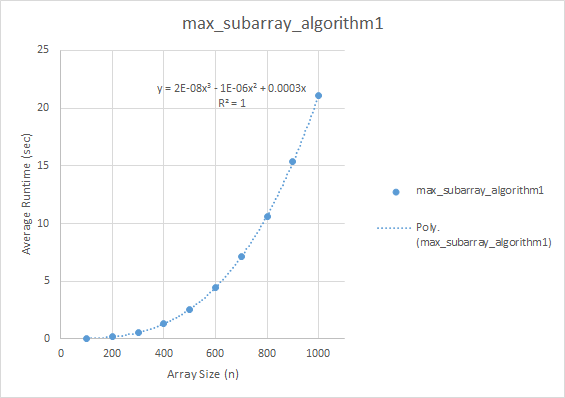
\includegraphics[width=\textwidth]{algo1Plot}
\begin{enumerate}[label=\bfseries Algorithm \arabic*:]
    % Algo 1
    \item \hfill \\
    \begin{description}
        \item[Experimental Run-time Function] \hfill \\
        \item[Biggest n in an hour] \hfill \\
    \end{description}

    % Algo 2
    \item \hfill \\
    \begin{description}
        \item[Experimental Run-time Function] \hfill \\
        \item[Biggest n in an hour] \hfill \\
    \end{description}

    % Algo 3
    \item \hfill \\
    \begin{description}
        \item[Experimental Run-time Function] \hfill \\
        \item[Biggest n in an hour] \hfill \\
    \end{description}

    % Algo 4
    \item \hfill \\
    \begin{description}
        \item[Experimental Run-time Function] \hfill \\
        \item[Biggest n in an hour] \hfill \\
    \end{description}
\end{enumerate}
\end{document}
%-------------------------------------------------------------------------------


